\RequirePackage{filecontents}
\begin{filecontents}{ref.bib}
@article{dey2014algorithm,
  title={Algorithm for Multi-Hand Finger Counting: An Easy Approach},
  author={Dey, Sumit Kumar and Anand, Shubham},
  journal={arXiv preprint arXiv:1404.2742},
  year={2014}
}
@article{chen2003hand,
  title={Hand gesture recognition using a real-time tracking method and hidden Markov models},
  author={Chen, Feng-Sheng and Fu, Chih-Ming and Huang, Chung-Lin},
  journal={Image and vision computing},
  volume={21},
  number={8},
  pages={745--758},
  year={2003},
  publisher={Elsevier}
}

@article{banerjee2014mouse,
  title={Mouse control using a web camera based on colour detection},
  author={Banerjee, Abhik and Ghosh, Abhirup and Bharadwaj, Koustuvmoni and Saikia, Hemanta},
  journal={arXiv preprint arXiv:1403.4722},
  year={2014}
}

\end{filecontents}
\documentclass{report}
\setcounter{secnumdepth}{3}
\usepackage{graphicx}
\usepackage[round]{natbib}
%\usepackage[backend=biber]{biblatex}
%\addbibresource{bib.bib} % with extension


\begin{document}

\author{Hamid Shayestehmanesh}
\title{Creating an Instrument Based On Movements in Webcam View}
\maketitle
\tableofcontents
\newpage

\chapter{Main Project Idea}
The main idea in this project is to build a HCI(Human Computer Interaction) application which can shape the music and users can draw it. In other words, we want to design and build an application which is able to translate hands gestures to meaningful sounds and build a new electronic music instrument.

\section{More Specified}
The goals of this project is to design an architecture of such application and build a prototype to detect hands and their movements. To do so, we use different colored cameras and regular speakers are used to generate sounds. Devices and implementation environment will be discussed in details later.
\pagebreak


\chapter{Literature}
This chapter is the most important chapter in this report. This section tries to translate required knowledge of music from musician language to computer scientists language thus, they can use this information to build different applications related to music.
\section{Music Language and Important Information}
Any system of signs and words that are used by a particular group of people to communicate and transfer knowledge about a specific subject is called a \textbf{language}. Nowadays, translation has become very common but, it faces variety of difficulties. Finding the best word in destination language, demonstrating emotions, feelings and, keeping the structure of the article are some of the hardest problems of translating. Here, we are trying to translate language of a musician to an engineer one. So, we will explain different important aspects of musical notes or music language which are mandatory to know about, while building a new instrument. To achieve our goal we explain what is the note language and state it in engineering form to find out what are important to compose and play a song. 

\subsection{Note Language}
Note language like other languages contains some specified signs which works as it's letters and they are written in lines. Human languages are usually written in a line with a few lane however, note language has 5 lanes which are very important. Each note has an actual sound, a length of time and power. 
\begin{itemize}
\item[Octave: ]{Octave of a note is determined by its place on the lanes. It's determined by the start place and end place of the note vertically. For example in \ref{fig:notes} third note starts in lane 2 and ends in lane 4 or first note starts in lane 1 and ends in lane 6 however the lane is not demonstrated.

\begin{figure}
\centering{ 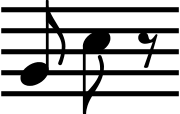
\includegraphics[width=1in]{180px-Eighth_notes_and_rest.png}}
\caption{The green color was separated to detect the point}
\label{fig:notes}
\end{figure}


}
\item[Note: ]{Notes are determined as the same as octave. Actually the vertical place shows note and octave together.}
\item[Octave and Note: ]{Octave and Note are used together to find out the exact frequency that the music should be played in. To be more specific octave show us range of frequency and Note show the exact frequency in the range.}
\item[Length of Time: ]{In the note language length of time is handled by the shape of a  note. Any article in note language has a base time and each note means a ratio over the base time. For example, \textbf{Eighth note} 
%\textit{reference be chang} 
is $1/2$ of base time. If the base time of a music is 10ms then this note means 5ms therefore, the player will play a frequency specified by the place of the note for 5ms.}
\end{itemize}
However with knowing time and frequency of each note this is possible to write a meaningful song but there's some more basic operators which can make a simple music to complex one.
\begin{itemize}
\item[Additional Signs on Notes: ]{Except the frequency and length of a note we should also determine how loud should it be played. Looking deep in music we can find this is meaningless to give each note a number or sign to demonstrate the loudness value. This would make the language very complex and also we should define loudness with measurable variable which is actually hard to understand for a musician. Musician mostly decides by intuition thus, they don't like counting! The language notifies the instrumentalist to play louder or more quite and also it shows where is the pick and how loud the pick is. In engineering aspect it may seem very obvious what to do when jumping to next note. You subtract your measure of current loudness from the pick and then divide it by the number of jumps but, it is not that simple in reality. As mentioned we are trying to design and implement a prototype so we will skip this part to keep it simple. }
\end{itemize} 
Talking about loudness, this should be mentioned that loudness is different to harshness. When we make a music louder the frequency and length and the feeling doesn't change but when we make a music harsher we change the way it is and the feeling it ignite in listener.s In a better word the feeling of the music can change it completely. We skip the feeling too.\newline
Addition to frequency, length and loudness of a note many other things can be obtain from note language like Bemol, Diez or Dot. We will omit more information of the language as they actually give advanced data about these three principles or how to acrobat between them. They will complicate our job however it may have no gain for us right now.


\iffalse
octave : ja nesbat be khootoot
note : ja nesbat be khootoot
time : shekl, nesbat be time avalie - agar noghte dasht mishe 1.5 barabar
frequency : octave and note
fasele hashoon : sefr hast
diez (nim parde bala) :
bemol (nim parde paeen) : 
agar ba khat beham vasl shodam vasleshoon mikone va note ro kamel tamoom nemikoni baddi ro shoro mikoni
agar nadasht ye chos mesghali fasele dare!
bolandi seda : ye seri shekl roie sareshoon
takid : bazam shekl roosh


meta data:
	speed = 250 masalan hast, ke clock ba estefade az metronom moshakhas mishe.

just this!
anything else Sara ?
\fi


\section{Meta Data}
Each music written in note language has some meta data. This meta data includes the speed of the song or in other words how long should a note with one unit of time takes. What should the feeling of the musician be? A few other information exists but they have no important effect on our architecture and job. 


\section{Conclusion}
To conclude from an engineer approach, to play a song we need to know frequency, length and loudness of each note of a song and also this have some different ways to move from a frequency and loudness to another frequency and loudness. The system must be able to move fast or smoothly. 


\chapter{Architecture}
As we discussed we at least need three different inputs to collect enough information to play a note and a core is necessary to convert this information to appropriate sound. Following figure demonstrate the situation.


\pagebreak
\chapter{Implementation}
During this chapter, first the prototype is discussed, then we will discuss one advanced input. 

\section{Prototype}

\subsection{Abstract}{A minimal model is implemented using Python, OpenCV and Pygame based on our proposed architecture. In this model there is an element detected by camera which frequency and amplitude is computed based on its coordinates. Coordination of the element identifies by color segmentation.}

\iffalse
Vertically changes the frequency of sound and moving it horizontally changes sounds' amplitude
complete the prototype part and 
\fi

\subsection{Prototype}
The prototype works with one specific element. The idea is to determine coordination of the object and use it as inputs. To find the element coordinates, we use color segmentation, in other word, we convert every pixel to black except those have a color with some special characteristics. Filtering the color or color segmentation will give us a black and white image which everything should be black but the element due to the fact that it is built in one particular color. In practice some other small areas will be converted to white. See figure \textbf{figure folan! noise! fogire az 2 3ta az hamina ke noise dashte bashe.} To solve this problem we add a noise reduction procedure after getting the black and white image. Erosion(\ref{ssec:erosion}) and Dilation(\ref{ssec:dilation})  the image will fairly solve the noise problem. By performing Erode and Dilate functions(Opening) small white pieces will be removed

\begin{figure}
\centering{
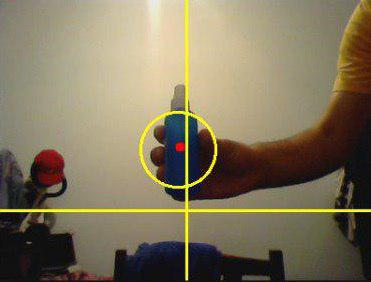
\includegraphics[width=1.4in]{blue1.jpg} 
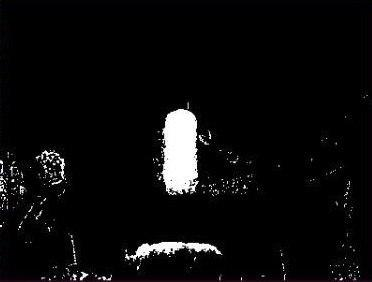
\includegraphics[width=1.4in]{blue2.jpg} 
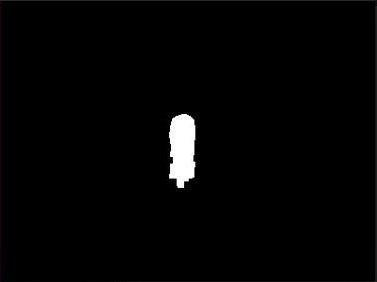
\includegraphics[width=1.42in]{blue3.jpg} }
\caption{(left)Original frame (middle) Color segmented frame (right) After opening.}
\label{fig:blue}
\end{figure}
 
  It will also remove around the element part which may turn it to a few parts. Dilating is used to merge the main white unit if it's affected by the Erode function. In next step we should identify the element by one point to track it's movements. To detect the center of element, first draw a contour around each white color region. As a contour won't usually have a good shape, find the minimum circle around the contour. This makes a good representation of the element coordination in image. Choose the biggest circle if there is more than one contour. Also the center of circle is a good \textit{one-point} identifier. \newline
Next, by comparing two last center of this imaginary circles can help us detect any movement of the element. Now that we have coordination and movement, we can update our frequency and amplitude. Generate and play a sound with specified frequency and amplitude using Pygame. Moving vertically changes frequency of sound and move it horizontally change sounds' amplitude.  \newline

\section{Object Tracking}
As mentioned we need to detect and follow an object in camera streams. In this section we will demonstrate how and why the object is evolved. We will discuss each element one by one and explain their flaws.

\subsection{Try 1}
The first two objects are recognized by their size and color in frames. The problem with these objects is that if any object with the same color appears in the frame and has an appropriate size, the system may follow the wrong object. So the system is not robust.

\begin{figure}
\centering{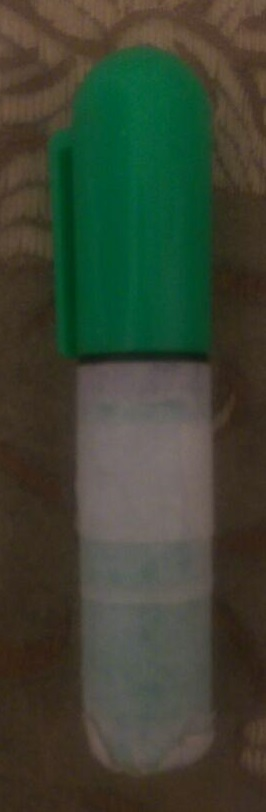
\includegraphics[width=1in]{Object1.jpg}
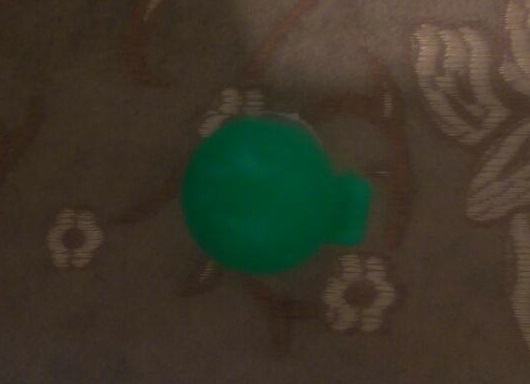
\includegraphics[width=2in]{Object1-2.jpg}}
\caption{Object1(try 1) Used from top (right image)} 	
\end{figure}

\subsection{Try 2}
One easy idea to solve the problem is to increase the size of the object. This way it becomes the largest object and must be recognized easier.

\begin{figure}
\centering{	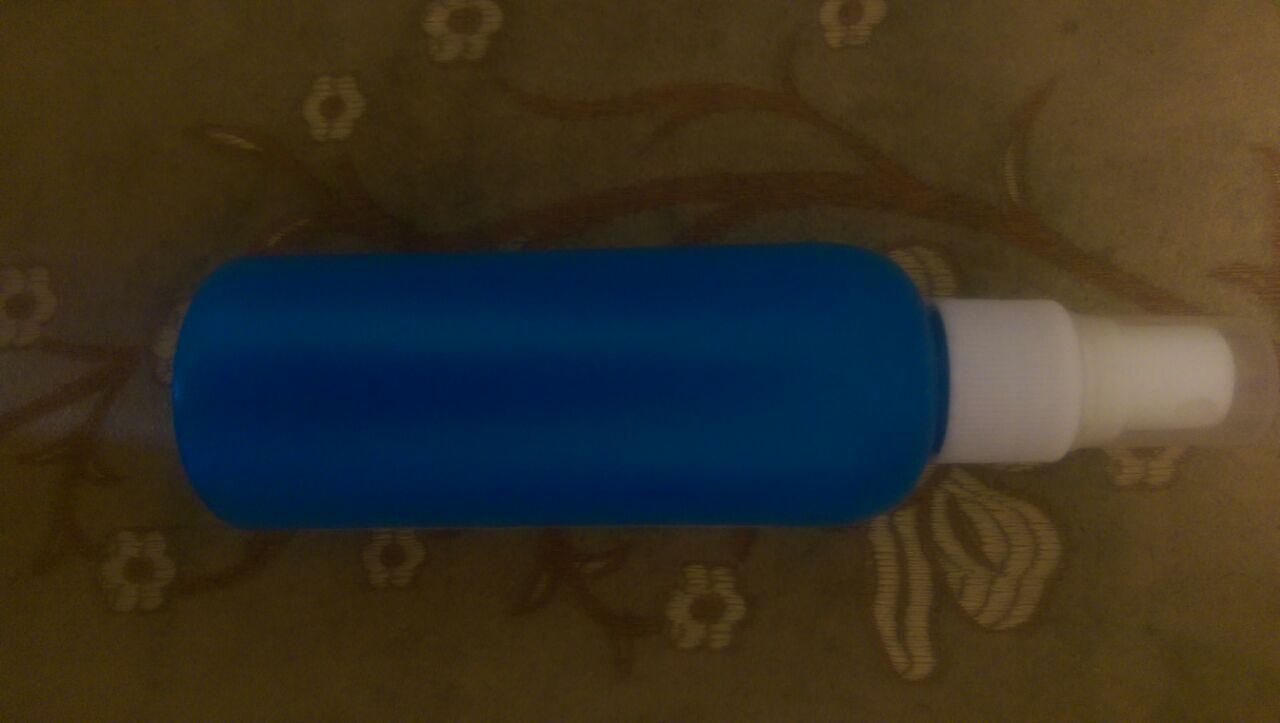
\includegraphics[width=3in]{Object2.jpg}  }
	\caption{Object2(try 2) - Used from side}  
\end{figure}
\begin{figure}
\centering{
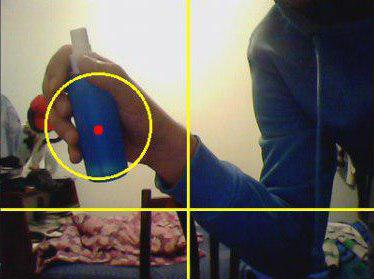
\includegraphics[width=1.4in]{bnoise1.jpg} 
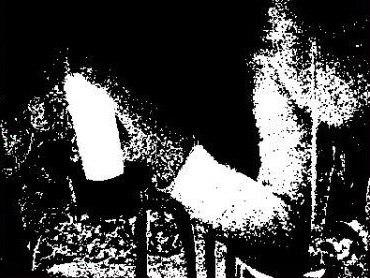
\includegraphics[width=1.4in]{bnoise2.jpg} 
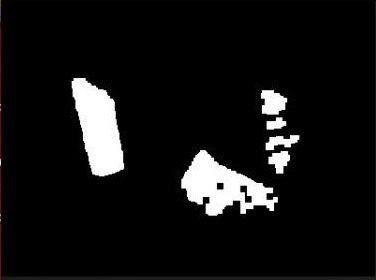
\includegraphics[width=1.42in]{bnoise3.jpg} }
\caption{(left)Original frame (middle) Color segmented frame (right) After opening - the system cannot decide which contour is the object.}
\end{figure}
Due to the fact that this step still recognize the object by size and color increasing the size won't help, mostly because of noises, sometimes the contour around the detected color becomes small specially in fast pace movements. Also increasing the size of the object has two consequences, first due to big size of the contour around the detected object it cannot move upon one direction much. It's shorter than what it should be. A little noise can change the center's coordination too much and make the system very vulnerable to noise. To sum up, an element with this size is far from practical. 
\subsection{Try 3}
In next attempt we need to resize the element and one idea to solve the size problem is to create a local background, therefore the colored point won't be lost in the background color. First attempt with this idea is one stick on hand. \newline

\begin{figure}
\centering{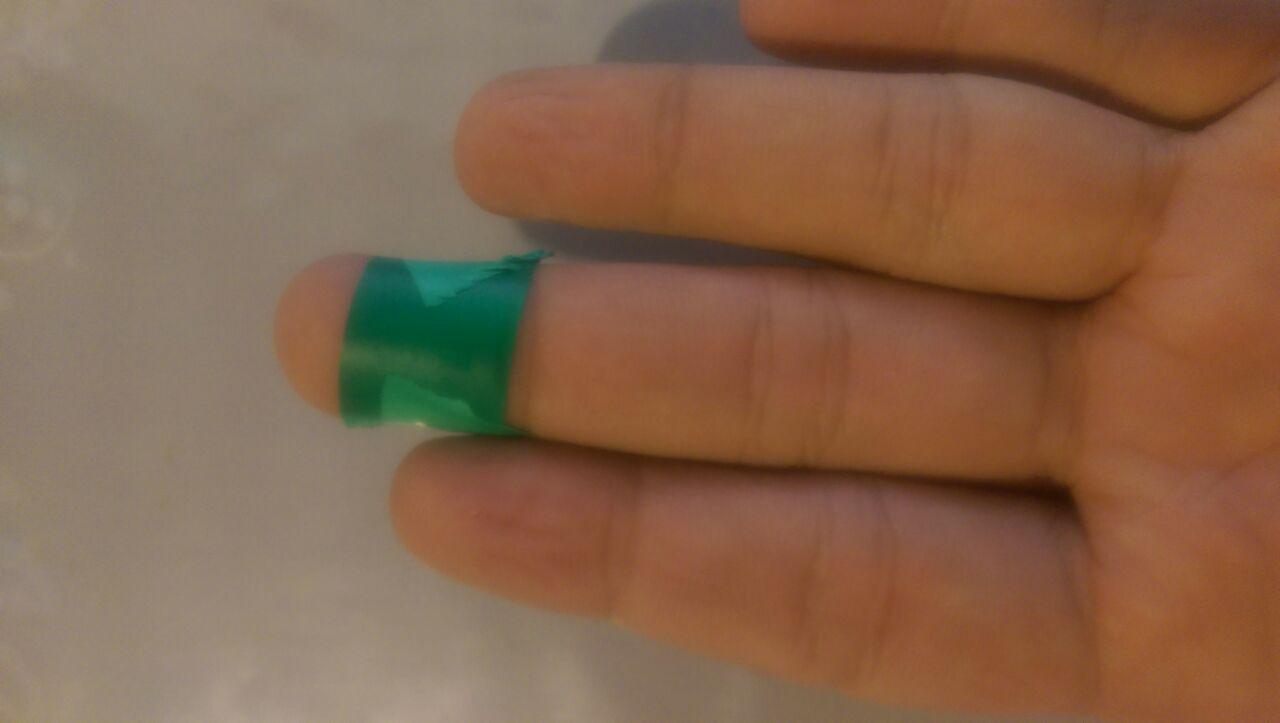
\includegraphics[width=3in]{Object3.jpg}}	
	 \caption{Object 3(try 3) - The green color was separated to detect the point}
\end{figure}


\subsection{Try 4}
Even though a green stick on the finger seems detectable but in practice the color of skin is not very stable so it isn't very helpful as a background, also light has an enormous effect on the color.
\subsection{Try 5}
To solve the problem some red stick are added up and down and then on left and right. Even the system works fine with only  up and down red sticks but adding left and right ones will help the system when very bright lights exists in the frame and makes it more robust to light.

\begin{figure}
\centering{	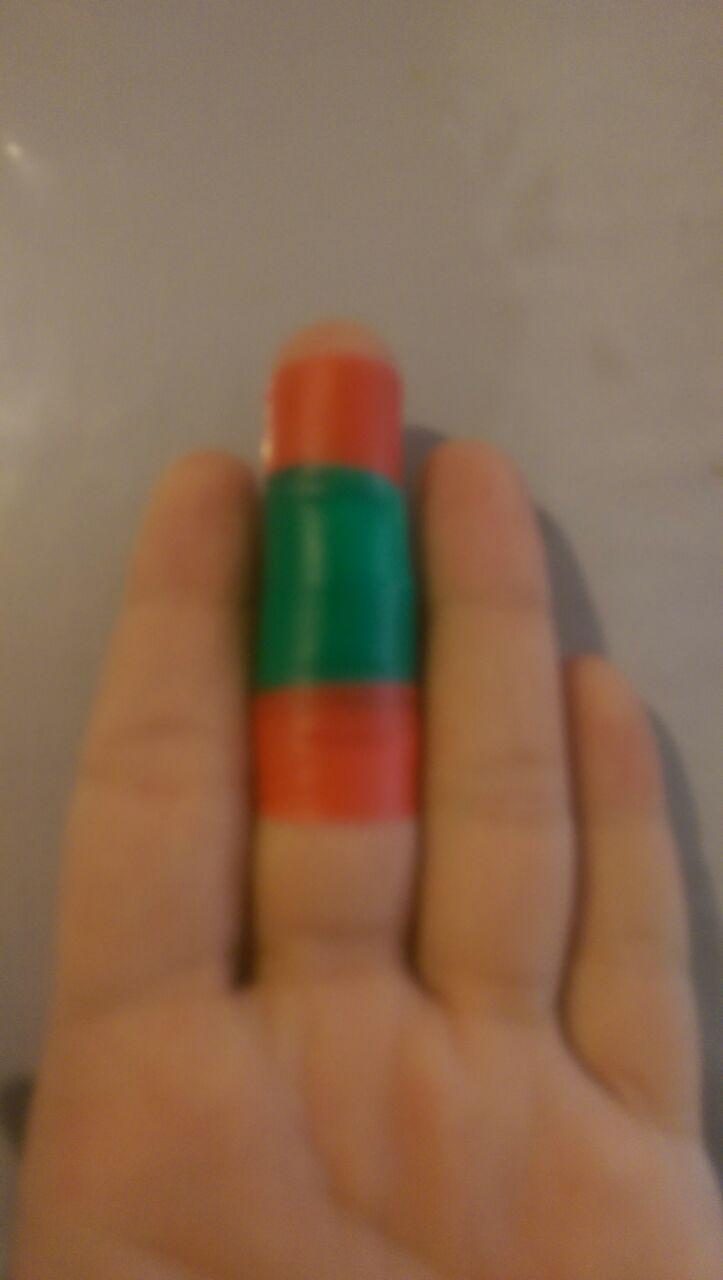
\includegraphics[width=2in]{Object4.jpg}  
	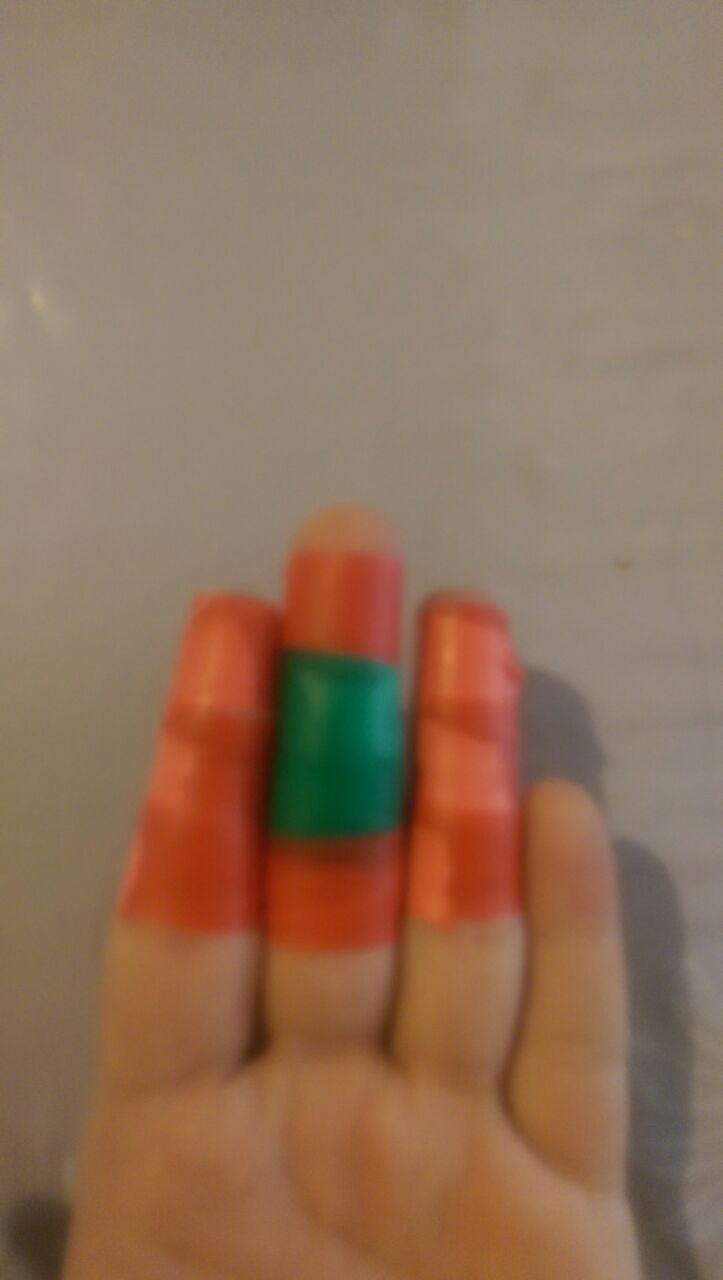
\includegraphics[width=2in]{Object5.jpg} }
	\caption{Try 4, 5}
\end{figure}

Due to the fact that sticks are very annoying on hands I created something with papers.

\begin{figure}
\centering{	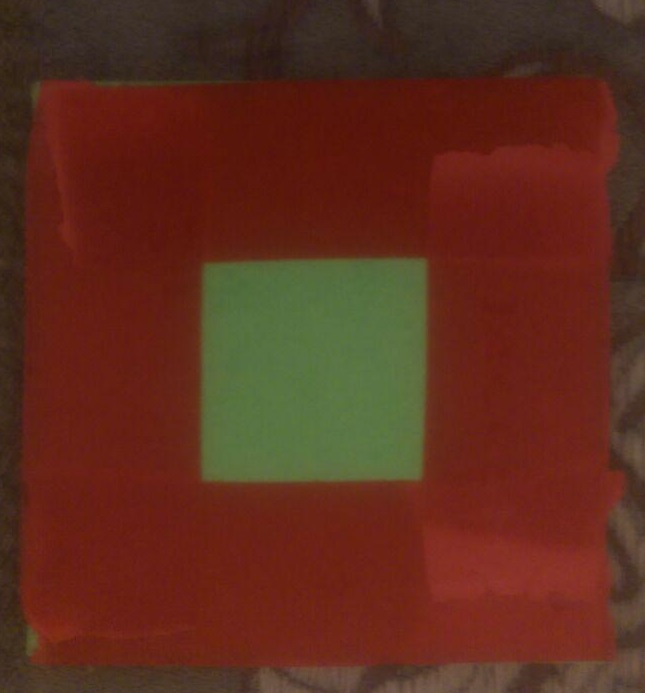
\includegraphics[width=2in]{Object6.jpg} }
	\caption{Created with papers, Try 6}
\end{figure}


\subsection{Try 6}
The papered object worked fine but because of the small background sometimes following the point became hard. To solve the problem we use the fact that one's hand won't move very fast, so if name current position of point $p_1 = (x_1, y_1)$ and next position $p_2 = (x_2, y_2)$ then the distance between $p_1, p_2$ is less than a constant $C$. So if we know the place of object's center, so we don't have to search the hole next frame to find the point. We have to search only a part of it. A square with upper left point of $p_1 - (C, C)$ and the lower right point of $p_1 + (C, C)$ seems adequate to search. With this object the system works very find and follows the target very well but it is common to lose the target in sharp lights.
\subsection{Try 7}
If we could ever make the background bigger to omit sharp lights more, the system could work in more complex situations. We created a glove with a circle on it. The big background it creates around the circle and the local square search mentioned in try 6 helps the system to track the point very well even if sharp light exists. 

 Different colors like, blue, black, white, light red, dark red were test as glove and the best color to use as a local background for a green circle is dark red. Not a very standard evaluation has been done to choose it. Colors have been test by sticking a green color on them and them using the system and then the best color has been chosen by author(tester). 

\begin{figure}
\centering{
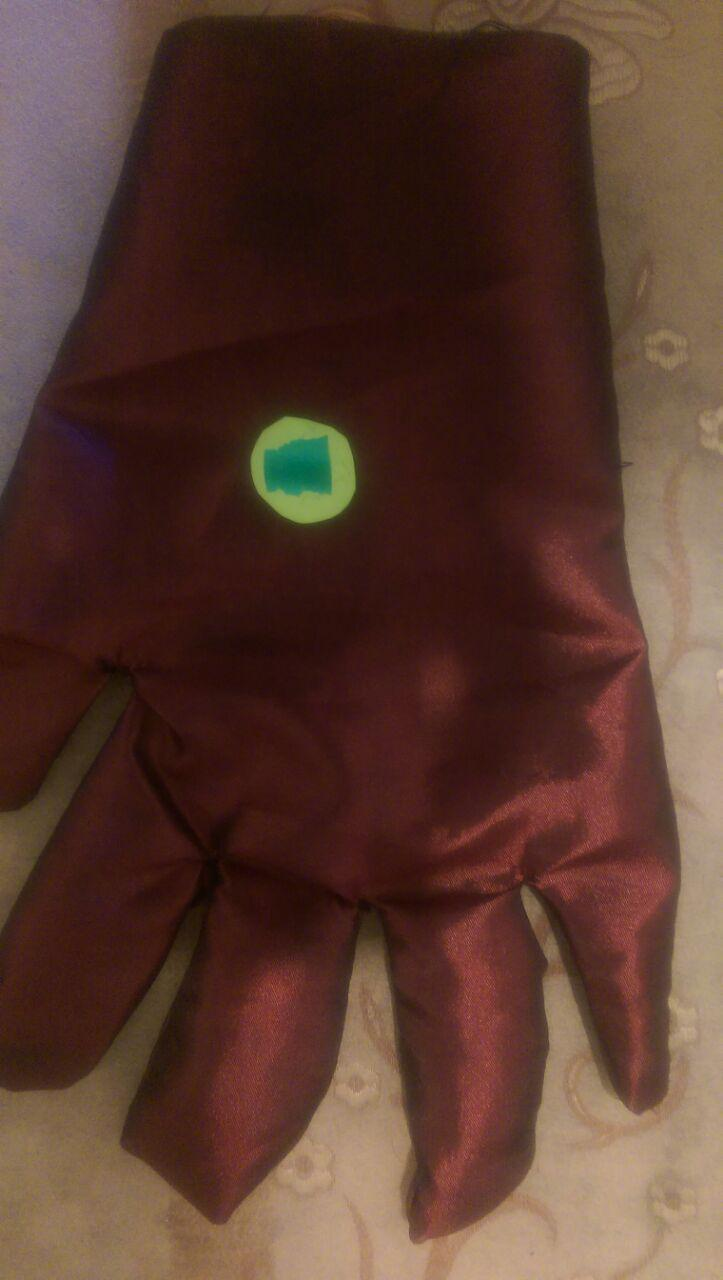
\includegraphics[width=2in]{Object8.jpg}
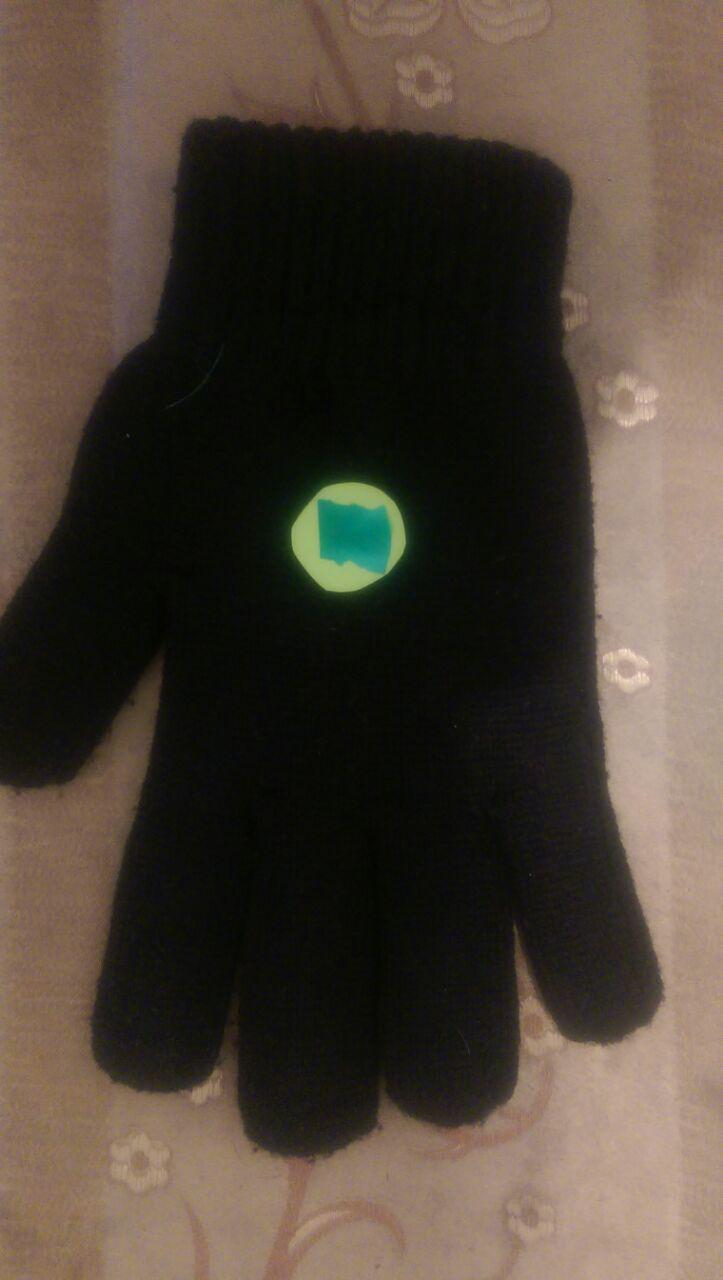
\includegraphics[width=2in]{Object7.jpg}}
\caption{Try 7, best color to be used with green is dark red.}
\end{figure}
	

\section{Playing Notes}
To play notes we break the frame into 6 parts, for 6 different notes. Shown below. Each .2 seconds the place of object is detected and a new note based on object coordination will be played. (In real implementation only one note plays.) A better split can be a partition to 9 parts like the one below.

\section{Counting Number of Open Fingers}
As we discussed an instrument needs a few different inputs. HCI
is the term used to refer the technologies that have been developed for interacting with machines \cite{dey2014algorithm}. As commonly instruments play with hands we want to focus on one bare hand input. Number of open fingers can be an input to choose the note or the amplitude. This algorithm will work based on \cite{dey2014algorithm} steps. But some steps are completely or partially changed. If there is more than one hands in an image our BFS-based algorithm is capable of working well.
\subsection{Method}
We can sub-divide the whole procedure into small manageable fragments described as below.
\begin{enumerate}

\item{Hand extraction}
\item{Noise reduction}
\item{Calculation of Centroid and orientation}
\item{Remove Unneeded Parts}
\item{BFS algorithm to count fingers}
\item{Update class zero, one and two}
\end{enumerate}
\subsection{Hand Extraction and Noise Reduction}
To extract the hand we do have some assumption and use three different methods and combine their result together to have a better hand result. In this part we are trying to obtain the best image of the hand for rest of our algorithm but, the exact shape of a hand. For example, assume a hand with fat fingers. Two adjacent fingers may stick together when those are open; which is not appropriate for our algorithm. We like a firm space between two neighbor fingers so those may not be detected as one. We use color skin segmentation, edge detection and background elimination to find and extract the hand. Before working on extraction we need to improve our image brightness so we perform histogram equalization on each frame. This will help to get a better result in environment with sharp lights. 
% bayad behtar beshe vase inke agar noor ziad bashe chizaie badi etefagh miofte. vase sade kardan rang 0 behtar kardan vaziat noor hast
\begin{enumerate}
	\item[Color Segmentation]{A very good explanation of skin color is $B \le G \le R$ \cite{chen2003hand} in a RGB pixel. The big problem with this solution is that it may detect some other stuff like a wooden case in the background or users yellow T-shirt. We call color segmented frame C1 .}
	\item[Background Elimination]{In this method first we obtain the background and then we eliminate it from frames containing hand. This will reach to the hand and other new objects in the frame. \cite{dey2014algorithm} uses the first frame as the background which won't work properly with all cameras because common cameras need a second to demonstrate the frames stably. Usual some first frames are to shiny or dark to be used as background but after some frames (50 frames for here) it is stable and can be used as background.(B1)  
	\begin{figure}
	\centering{
\includegraphics[width=1.2in]{1.jpg}
	
\includegraphics[width=1.2in]{50.jpg}
	\caption{frame number 1 and 50. frame 50 is more stable however the scene has no change. }}
	\end{figure}
	} % vase gereftane background bayad 3seconds 150 ta frame aval ignore beshe. bekhatere inke chize khoobi azash dar nemiad. va masalan rang va noor khoob nist. mesal az frame aval va frame akhar. albate in rabt be camera ham dare. 
	\item[Edge Detection] {First edges in background are determined and then edges from current frame and edges in current frame which do not exists in background are left in a frame called E1. Canny function is used to extract edges.}
\end{enumerate}
Then these three frames are converted to binary black and white images. Then we call D1 as logically or function of E1 and A1 where A1 is logically and of C1 and B1. Finally result is cleaned by Erode and Gaussian function. 
\textit{some figure of left images}


\subsection{Calculation of Centroid and Orientation}
Finding Orientation is an important factor in the algorithm as it helps the algorithm to be valid
even if the hand is placed slightly inclined or slanted rather than in the ideal upright orientation. A very simple and basic approach has been followed to find the orientation of the hand. 
\subsubsection{Calculating centroid} \label{sssec:cc}
We calculate centroid of the white pixels by finding the spatial mean along x and y direction by
giving equal unity weights to each pixel.
$$ Centroid(x, y) = \Sigma x_i / n, \Sigma y_i / n  $$
Where, $x_j$ and $y_i$ represent the x and y coordinates of the pixel in row i and column j. Total
number of pixels are represented by n.
\subsubsection{Calculating orientation}
We use a line that gives us the idea about the orientation of the hand. If we show our hand with
open palm to the camera such that our middle finger points vertically upwards, then the line
perpendicular to our hand, which happens to be the horizontal line in this case, can be termed as
base line. Here on, the base line will be used to refer the line which is perpendicular to the hand or to any part of it. \newline
To find the base line, we take the centroid of all points of hand that happen to lie on the lowest
horizontal line. Then we find the line joining this centroid to the centroid of the hand that we
found in section \ref{sssec:cc} Let that line joining the two centroids be represented by $y = m_1.x + c_1.A$
line perpendicular to this line will have slope of ($-1/m_1$ ). This line, if has to pass through the
centroid of lowest horizontal line $(x_{cb} , y_{cb} )$, will have the equation as
This line intersects the hand almost perpendicularly and here we get our first base line. It roughly
replicates the orientation of the hand within the range of $-45 to +45$ degree from vertical axis\cite{dey2014algorithm}.  

\subsection{Remove Unneeded Parts}
To decrease complexity of next steps and centralize our detail we remove all fully black rows and columns. Then we remove the palm and arm if any of that exists. To remove the palm we perform following algorithm.
\begin{enumerate}
\item{First get the average of 5 bottom rows white pixels and call it C.}
\item{Remove bottom 5 rows.}
\item{While most bottom row's number of white pixels is more than $.95 * C$ then }
\item{Update C by number of white pixels of most bottom row.}
\item{Remove the most bottom row.}
\end{enumerate} 

\subsection{BFS-based Algorithm to Count Fingers}
To count the number of open fingers we use the fact that the top point of an open finger is considerably above of rest of the hand. So we start from the top row and move down to find the first line having white pixels. This means we have found a finger so we remove this finger and repeat the algorithm till there is some white pixel on the image. To remove the finger we perform following algorithm 
\begin{enumerate}
	\item{Color current pixel as black}
	\item{repeat from left/right/bottom pixel if white}
\end{enumerate}
regardless of fingers orientation, it is removed after running mentioned algorithm. After first run(removing first finger) hands palm is removed too. But, when no finger is open there is at least one starting point to remove the white pixels. Also as shown in figure \ref{fig:twostarts} hands with one open finger are usually fully cleaned with two starting points rather than one. 
\begin{center}
\begin{figure}
\centering {
\includegraphics[width=1in]{one.jpg}}
\caption{Two starting points for one open finger}
\label{fig:twostarts}
\end{figure}
\end{center}

\subsection{Update Class Zero and One}
As we discussed we expect our algorithm to detect one open finger as two and zero open finger as one therefor, we should find a way to decrease the mistake. Too detect the false negative answers of class two we focus on y-dimension distance of two starting points. If the answer is really two then these two starting point are almost near each other otherwise they are more distant. A threshold of 15 pixels is good value to detect false negative samples. If x-distance of these two starting points is more than 15 then there is only one open finger. \newline
To classify zeros from one we use the fact that all the columns in zero image have almost same white pixels. First we find the maximum and minimum white column. If min and max difference is more than 40 then there is one open finger otherwise no open finger exists.
\begin{figure}
\centering {
\includegraphics{two_distance.jpg}}
\caption{Distance of starting points is very shorter when only one finger is open.}
\end{figure}
\begin{figure}
\centering {
\includegraphics{zeros.jpg}}
\caption{Shortest and longest white column is zeros are most in same range.}
\end{figure}


\subsection{Performance Analysis}
We tested on three individuals with different palm sizes. \newline
\centering{\begin{tabular}{|l| c| c| c| c| c|} \hline
  Datasets & 0 finger & 1 finger & 2 fingers & 3 fingers & 4 fingers  \\ \hline
  Dataset 1 & 1 & 0.86 & .93 & 1 & 1  \\ \hline
  Dataset 2 & 1 & 0.86 & 1 & 1 & 0.88  \\ \hline
  Dataset 3 & 0.66 & 0.9 & 0.95 & 1 & 0.86  \\ \hline
\end{tabular}
}
The reason only four fingers are presented in test and tomb is remove is that if we open the tomb finger downward then it will be remove while removing the palm or when we are removing the first finger. If it's opened upward the finger removing won't hurt tomb, but still it may be removed by palm removal.
\section{Conclusion}
We intended to develop an algorithm as input for the architecture and implementing a prototype. The finger counting algorithm has great amount of flexibility and thus can be used for numerous applications with accurate results. \newline We proceeded with few assumptions. Firstly we assume that the hand is shown from bottom of
the image such that fingers lie on relatively upper part of the image with respect to the rest of the
hand.
We successfully used the algorithm to count up to four fingers under the resolution of 800x600 obtained from Xiaomi Redmi3 prime using Ip webcam application. 

All the codes was written in Python with OpenCV and they were tested on a
machine featuring Intel Core I7-2670 3.0GHz processor and 12GB RAM on Ubuntu 14.04
platform. We used Xiaomi Redmi3s Prime's front camera which is a 5MP, connected using Ip Webcam application for finger counting algorithm and a 2MP built in webcam on Lenovo Z570 is used for first part.
With finger counting algorithm we can trigger 5 unique commands. By adding second hand it is increased to $5 \times 5 = 25 $ and can support at least three octave that each one contains seven notes.


\chapter{Important Functions and OpenCV}
\section{Erosion and Dilation}
\subsection{Erosion} \label{ssec:erosion}
The basic idea of erosion is just like soil erosion only, it erodes away the boundaries of foreground object (Always try to keep foreground in white). So what it does? The kernel slides through the image (as in 2D convolution). A pixel in the original image (either 1 or 0) will be considered 1 only if all the pixels under the kernel is 1, otherwise it is eroded (made to zero).

So what happens is that, all the pixels near boundary will be discarded depending upon the size of kernel. So the thickness or size of the foreground object decreases or simply white region decreases in the image. It is useful for removing small white noises (as we have seen in color space chapter), detach two connected objects etc.
\subsection{Dilation} \label{ssec:dilation}
It is just opposite of erosion. Here, a pixel element is ‘1’ if at least one pixel under the kernel is ‘1’. So it increases the white region in the image or size of foreground object increases. Normally, in cases like noise removal, erosion is followed by dilation. Because, erosion removes white noises, but it also shrinks our object. So we dilate it. Since noise is gone, they won’t come back, but our object area increases. It is also useful in joining broken parts of an object.
\subsection{Opening}
Opening is just another name of erosion followed by dilation. It is useful in removing noise, as we explained above. Here we use the function, cv2.morphologyEx().
\subsection{Closing}
Closing is reverse of Opening, Dilation followed by Erosion. It is useful in closing small holes inside the foreground objects, or small black points on the object.

\textit{$http://docs.opencv.org/3.0-beta/doc/py_tutorials/py_imgproc/py_morphological_ops/py_morphological_ops.html$}

\section{cvtColor}
The function converts an input image from one color space to another. In case of a transformation to-from RGB color space, the order of the channels should be specified explicitly (RGB or BGR). Note that the default color format in OpenCV is often referred to as RGB but it is actually BGR (the bytes are reversed). So the first byte in a standard (24-bit) color image will be an 8-bit Blue component, the second byte will be Green, and the third byte will be Red. The fourth, fifth, and sixth bytes would then be the second pixel (Blue, then Green, then Red), and so on.

\chapter{Other Technologies and Future Work}
\begin{itemize}
\item{A programming language called Chuck has been created in Princeton university. ChucK is a programming language for real-time sound synthesis and music creation. The problem with this language is that it's doesn't support any library which can use webcam or any type of camera, neither easy way to connect it to another programming language.}
\item{Adding a step to bfs-based algorithm to detect hands and split them. So the hole algorithm can work for multiple hands.}
\item{Improving second phase part to update class one and zero.}
\end{itemize}

\bibliography{ref}
\bibliographystyle{plain}


\end{document}